\documentclass[11pt,a4paper]{article}
\usepackage{enumitem}
\usepackage{graphicx}           % Extended \includegraphics         
\usepackage[reqno]{amsmath}            % Higher mathematics
\usepackage{hyperref}           
\usepackage[margin = 0.5in]{geometry}
\usepackage{float}
\usepackage{amssymb}            % special math fonts
\usepackage{amsmath}
\usepackage{siunitx}
\usepackage{enumitem}
\usepackage{cancel}
\usepackage{braket}
\usepackage{tikz}
\usepackage{pgfplots}
\usepackage[final]{pdfpages}
\usepackage{physics}
\usepackage{subcaption}
\usepackage{bbm}
\usepackage{rotating}
\usepackage{listings}
\usepackage{color}

\makeatletter
\renewcommand*\env@matrix[1][*\c@MaxMatrixCols c]{%
  \hskip -\arraycolsep
  \let\@ifnextchar\new@ifnextchar
  \array{#1}}
\makeatother

\definecolor{codegreen}{rgb}{0,0.6,0}
\definecolor{codered}{rgb}{0.6,0,0}
\definecolor{codeblue}{rgb}{0,0,0.6}
\definecolor{codegray}{rgb}{0.5,0.5,0.5}
\definecolor{codepurple}{rgb}{0.58,0,0.82}
\definecolor{backcolour}{rgb}{0.95,0.95,0.92}
 
\lstdefinestyle{mystyle}{
    backgroundcolor=\color{backcolour},   
    commentstyle=\color{codered},
    keywordstyle=\color{codeblue},
    numberstyle=\tiny\color{codegray},
    stringstyle=\color{codegreen},
    basicstyle=\footnotesize,
    breakatwhitespace=false,         
    breaklines=true,                 
    captionpos=b,                    
    keepspaces=true,                 
    numbers=left,                    
    numbersep=5pt,                  
    showspaces=false,                
    showstringspaces=false,
    showtabs=false,                  
    tabsize=2
}
 
\lstset{style=mystyle}

%\tikzexternalize[optimize=false,prefix=PREFIX]

\pgfplotsset{compat = 1.13}

\newcommand{\h}{\hat}
\newcommand{\hham}{\hat{\mathcal{H}}}

\begin{document}


\title{\bf PHYC90010 - Statistical Mechanics Assignment 4}
\author{Mitchell de Zylva - 756539}
\maketitle



\begin{center}
\vspace{1cm}
\rule{145mm}{0.5mm}
\vspace{1cm}
\end{center}
\tableofcontents
\newpage
%\input{/home/part3/mylatex/preamble}
\newpage

\includepdf[pages=-]{/home/mitchell/Documents/masters/statmech/fourth/Assign4_2019.pdf}


%%%%%%%%%%%%%%%%%%%%%%%%%%%%%%%%%%%%%%%%%%%%%%%%%%%%%%%%%%%%%%%%%%%%%%
\section{Question 1 }
\label{sec:question1}
%%%%%%%%%%%%%%%%%%%%%%%%%%%%%%%%%%%%%%%%%%%%%%%%%%%%%%%%%%%%%%%%%%%%%%
%%%%%%%%%%%%%%%%%%%%%%%%%%%
\subsection{Question 1 - (a)}
\label{sec:question1:subsec:parta}
%%%%%%%%%%%%%%%%%%%%%%%%%%%
We begin by considering the equation that defines the dynamics of the budworm population
\begin{equation}\label{eq:dynamics}
\pdv{u}{t} = \left[ ru \left( 1 - \frac{u}{k} \right) \right] - \frac{u^2}{1+u^2} + D \nabla^2 u
\end{equation}
Since we are looking for stationary solutions, we need to set $\pdv{u}{t} = 0$, and the requirement that they be uniform solutions means that we can assume $\nabla^2 u = 0$. This transforms the equation
\begin{align*}
0 &= \left[ r u \left( 1 - \frac{u}{k} \right) \right] - \frac{u^2}{1 + u^2} \\
&= \frac{r u (1 + u^2) - r/k u^2 (1+u^2) - u^2 }{(1+u^2) } \\
&= r u + r u^3 - \frac{r}{k} u^2 - \frac{r}{k} u^4 - u^2 \\
&= u \left( r + r u^2 - \left( \frac{r}{k} + 1 \right) u  - \frac{r}{k} u^3 \right) 
\end{align*}
By the null factor law, this has a solution at $u=0$. Since we now expect there to be a trivial solution at $u=0$, we can compute the Jacobian for the system, where we define the function $F$ to be
$$ F =  \left[ r u \left( 1 - \frac{u}{k} \right) \right] - \frac{u^2}{1 + u^2}.$$
In this case, since there is only one variable, the Jacobian will only be $\pdv{F}{u}\rvert_{u=0}$, and so will only have one corresponding eigenvalue. 
\begin{align*}
\pdv{F}{u}\big\rvert_{u=0} &= \left[ \pdv{u} \left[ r u \left(1 - \frac{u}{k} \right) - \frac{u^2}{1+u^2} \right] \right]_{u=0} \\
&= \left[r - \frac{r u}{k} - \frac{r u}{k} - \frac{2 u}{(1+u^2)^2}\right]_{u=0} \\
&= r 
\end{align*}
Since $r >0 $, and it is the eigenvalue for the system at $u=0$,  we know that the growth of the function will drive it away from equilibrium, and so the trivial, uniform solution will be unstable.
%%%%%%%%%%%%%%%%%%%%%%%%%%%
\subsection{Question 1 - (b)}
\label{sec:question1:subsec:partb}
%%%%%%%%%%%%%%%%%%%%%%%%%%%
Now if we solve for the uniform stationary solutions again, we note that 
$$ 0 = u \left(\underbrace{ r + r u^2 - \left( \frac{r}{k} + 1 \right) u  - \frac{r}{k} u^3 }_{\textbf{A}}   \right)$$
Now, by Null Factor Law, we know that term \textbf{A} must also be equal to zero. This suggests that the system can have one, two, or three more possible solutions, depending on chosen values of $k$ and $r$. 

We know that a cubic must, by definition, have at least one real solution, but the behaviour of the other possible solutions can be real, or imaginary. We can see what conditions give this single solution by looking at the cubic discriminant. 
\begin{itemize}
\item $\Delta_3 > 0$, then the equation has three distinct roots.
\item  $\Delta_3 = 0 $, then the equation has three real roots, one of which is repeated. 
\item $\Delta_3 < 0 $, then the equation has one real root, and two non-real, complex conjugate roots
\end{itemize}
The discriminant of a cubic is given by 
$$ \Delta_3 = b^2 c^2 - 4 a c^3 - 4 b^3 d - 27 a^2 d^2 + 18 a b c d $$
for the standard form of the cubic, where we can see that in this case 
\begin{align*}
a &= \frac{-r}{k} ,\\
b &= r ,\\
c &= - \left( \frac{r}{k} + 1 \right), \\
d &= r.
\end{align*}
This makes the discriminant for this term into 
\begin{align*}
\Delta_3 = \frac{(-4 k^3 r - 12 k^2 r^2 + k^4 r^2 - 12 k r^3 + 20 k^3 r^3 - 4 r^4 - 
 8 k^2 r^4 - 4 k^4 r^4)}{k^4}. 
\end{align*}
This discriminant will have regimes where it will be positive, zero, and negative, suggesting that the corresponding cubic will provide either three, two, or one addition stationary solution.

%%%%%%%%%%%%%%%%%%%%%%%%%%%
\subsection{Question 1 - (c)}
\label{sec:question1:subsec:partc}
%%%%%%%%%%%%%%%%%%%%%%%%%%%
Now, we need to consider the possible values of $k$ and $r$. Since $r$ represents a birth rate, it must be real. Simillarly, since $k$ represents the competition, it must also be a real number. We also know that in  order for us to find the appropriate behaviour, we have to see where the graph of the cubic discriminant crosses $0$, since this is the point at which the number of real solutions will change. 

If we plot the behaviour of the discriminant in Mathematica, we see the following shape of the discriminant.
\begin{figure}[H]
\begin{center}
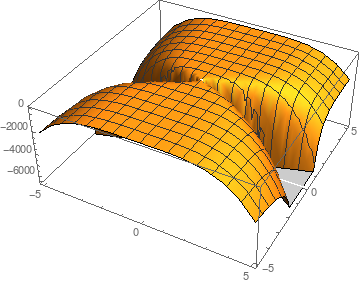
\includegraphics[scale=0.5]{/home/mitchell/Documents/masters/statmech/fourth/discriminant.jpg}
\caption{Cubic Discriminant $\Delta_3 $ as a function of $r$ and $k$}
\end{center}
\end{figure}
This is difficult to process, give the scale, so if we then consider the region where the discriminant is greater than 0 by taking a slice through the graph of the cubic discriminant $\Delta_3 = 0$, we see that it takes the form of 
\begin{figure}[H]
\begin{center}
\includegraphics[scale=0.5]{/home/mitchell/Documents/masters/statmech/fourth/Contour.jpeg}
\caption{Cubic Discriminant as a function of $r$ (vertical axis) and $k$ (horizontal axis)}
\end{center}
\end{figure}
Here we see the contour where the discriminant crosses 0. Anything highlighted in blue are points in the contour where the discriminant is greater than 0, anything on the line is equal to zero, and anything outside the line is less than zero. Therefore, if the values of $k$ and $r$ are in the blue section of phase space, there will be 3 stationary solutions provided by the cubic dicriminant, if it is on the boundary, it will provide 2 stationary solutions. If it is outside this area of phase space, it will be only provide one solution.

\textbf{Note:} I have considered cases above where the birth rate is relative, i.e. it can be negative when one takes into account the total birth rate minus the total death rate. Similarly I am considering cases where a negative competition means that resources are greater than the load on the system from the population. Should this not be the case, we can restrict the domain so that it only takes into account the first quadrant, where both $k$ and $r$ are positive. 
\begin{figure}[H]
\begin{center}
\includegraphics[scale=0.5]{/home/mitchell/Documents/masters/statmech/fourth/contour_2.jpeg}
\caption{Cubic Discriminant as a function of $r$ (vertical axis) and $k$ (horizontal axis)}
\end{center}
\end{figure}
This plot makes it look more like the contour asymptotes to 0, rather than having an absolute cut-off, but it is unclear if this is a product of Mathematica's plotting function. Therefore, the region where there is only one additional stationary solution, is the white region in Figure 3.
%%%%%%%%%%%%%%%%%%%%%%%%%%%
\subsection{Question 1 - (d)}
\label{sec:question1:subsec:partd}
%%%%%%%%%%%%%%%%%%%%%%%%%%%
If we now introduce diffusion, we can determine if the stability of the $u=0$ solution changes by treating the expression as a 1 dimensional logistic population with Fick Diffusion. If we assume that $u$ has the form of $u(x,t)$, we look for travelling wave solutions which have the form $u(x-ct)$. This makes \eqref{eq:dynamics} into, where primes denote $\pdv{\xi}$ where $\xi = x - ct$:
$$ - c u^\prime = \left[ ru  \left(1 - u/k \right) \right] - \frac{u^2}{(1+u^2)} + D u^{\prime \prime}. $$
Now if we let $v=u^\prime$, this becomes 
\begin{align*}
-cv &= \left[ ru \left( 1 - \frac{u}{k} \right) \right] - \frac{u^2}{1+u^2} + D v^\prime \\
D v^\prime &= \left[ -ru \left( 1 - \frac{u}{k} \right) \right] + \frac{u^2}{1+u^2} - cv \\
v^\prime &= \frac{1}{D} \left[ \left[ - ru \left( 1 - \frac{u}{k} \right) \right] + \frac{u^2}{1+u^2} - cv \right]
\end{align*}
Now linearising about the point $u=0$ and finding the Jacobian, we see 
\begin{align*}
J &= \begin{pmatrix}
\dv{u^\prime} & \dv{v^\prime} \\
\dv{u} & \dv{v}
\end{pmatrix}_{u_0,v_0} \\
&=\begin{pmatrix}
0 & D \\
-r & -c 
\end{pmatrix}
\end{align*}.
Finding the eigenvalues, we see that the characteristic equation is given by 
\begin{align*}
0 &= \det(J - I \lambda) \\
&= \begin{vmatrix}
-\lambda & D \\
-r & -c-\lambda
\end{vmatrix}\\
&= (-\lambda) (-c - \lambda) + rD
&= \lambda^2 + c \lambda + rD .
\end{align*}
This has solutions of the form 
\begin{align*}
\lambda &= \frac{- c \pm \sqrt{c^2 - 4 rD}}{2}.
\end{align*}
These solutions will be real when $c^2 - 4 rD  \geq 0 $, and this leads to when $c \geq \abs{2 \sqrt{r D}}$, the solutions will be negative. This suggests that the introduction of diffusion will cause the $u = 0 $ solution to become stable. 
%%%%%%%%%%%%%%%%%%%%%%%%%%
\subsection{Question 1 - (e)}
\label{sec:question1:subsec:parte}
%%%%%%%%%%%%%%%%%%%%%%%%%%%

%%%%%%%%%%%%%%%%%%%%%%%%%%%
\subsubsection{Question 1 - (e) - i}
\label{sec:question1:subsec:parte:subsub:i}
%%%%%%%%%%%%%%%%%%%%%%%%%%%
The boundary conditions $u(0,y) = u(L,y) = u(x,0) = u(x,L) = 0$ are appropriate because we have assumed that the forest is finite. From a mathematical standpoint, for a finite square forest, the population density must be normalised, and the presence of diffusion causes build up in at the edges of the forest, which would lead to the probability blowing up. If we allowed the diffusion to keep diffusing out the population, the boundaries would have to keep growing, effectively changing the system from finite to infinite. It also follows that since we are searching for uniform stationary solutions, since the boundaries are set to be 0, the rest of the solution must also equal zero. From a physical standpoint, it stands to reason that for we should not expect to find budworms outside the boundaries of their natural habitat, and once outside of the forest the conditions that describe their population density would be different from the conditions described in the question.

%%%%%%%%%%%%%%%%%%%%%%%%%%%
\subsubsection{Question 1 - (e) - ii}
\label{sec:question1:subsec:parte:subsub:ii}
%%%%%%%%%%%%%%%%%%%%%%%%%%%
This boundary is only compatible with the uniform stationary state $u=0$ because the moment you introduce any population density, in the presence of diffusion it will spread to the edges and be absorbed by the boundary. This means that any new population will eventually diffuse out of the system, and so the boundary conditions are only compatible with the state where $u=0$

%%%%%%%%%%%%%%%%%%%%%%%%%%%
\subsubsection{Question 1 - (e) - iii}
\label{sec:question1:subsec:parte:subsub:iii}
%%%%%%%%%%%%%%%%%%%%%%%%%%% 
For equation \eqref{eq:dynamics}, we want to see if there will be any stable pattern formation that is compatible with the solution $u=0$. To do this, we consider that the population density field has the same form as the general expression given in the notes:
$$ \pdv{u}{t} = \gamma f(u,v) + D \nabla^2 u $$
where $\gamma = 1$ and $f(u,v) = \left[ ru \left( 1 - \frac{u}{k} \right) \right] - \frac{u^2}{1+u^2}$. If we want a stable node at $f(u_0) = 0$, the Jacobian must be real and negative. Given that we have a single variable function, we can consider the Jacobian to be single valued, that is:
$$ A = \begin{pmatrix}
f_u
\end{pmatrix}_{u_0} = \left[r - \frac{-2r u}{k} - \frac{2u (1+u^2) - u^2 (1+u^2)}{(1+u^2)^2}\right]_{u=0}.$$
If we introduce a small perturbation of the form $ \textbf{W} = u - u_0 $, and linearising the equation, we have 
$$ \dv{\textbf{W}}{t} = \gamma A \textbf{W} + D \nabla^2 \textbf{W} .$$
If we assume that there is some time dependance proportional to $\exp{\lambda t}$, we can expand the spatial part as a complete set of eigenfunctions which satisfy the boundary conditions. These will be periodic functions, since the boundary conditions are periodic, and so we consider the case where 
$$ \nabla^2 W_\textbf{k}(x,y) = - (k_x^2+k_y^2) W_\textbf{k}(x,y) $$
Substituting this in, and using orthogonality in the same manner as in section 8.3.1 of the notes, this becomes 
$$ \lambda \textbf{W}_\textbf{k} = \gamma A \textbf{W}_\textbf{k} - D (k_x^2 + k_y^2) \textbf{W}_\textbf{k} $$
We know from lectures, that this equation has non-trivial solutions when 
$$ \det(\lambda - \gamma A + D (k_x^2 + k_y^2) )= 0 .$$
If we assume that the wave that propogates has the form of a 2D wave, we can claim that it will satisfy the condition $k_x \approx k_y$. Now, if we subsititute in our expression for $A$, taking $\gamma = 1$, this will be critical when $\lambda = 0$, and so we can say 
\begin{align*}
0 &= f_u\rvert_{u=0} - 2D k^2 \\ 
0 &= r - 2 D k^2 \\
k_c &= \sqrt{\frac{r}{2D}}
\end{align*}
If we know that the wave-vector is greater than the critical wave-vector $\textbf{k}$, then it will satisfy the condition given in lecture notes, and generalised for 2 dimensions
\begin{align*}
k_c &> k_{min} = \frac{\pi^2}{L^2} \\
\sqrt{\frac{r}{2D}} &> \frac{pi^2}{L^2} \\ 
\Rightarrow L &> \pi \left( \frac{2D}{r} \right)^{1/4}.
\end{align*}
This means that in order for there to be a non-zero population supported, the size of the forest must exceed $\pi \left( \frac{2D}{r} \right)^{1/4}$
\end{document}